% Paste into Section 5.2. Upload the three PDFs to figures/ in Overleaf.
% Uses graphicx and subcaption, both already loaded by the manuscript.
Figure~\ref{fig:paired_route_time} shows the difference in recorded route
duration between full and partial charging for the 43 base-case instances,
grouped by route class.

\begin{figure}[tbp]
    \centering
    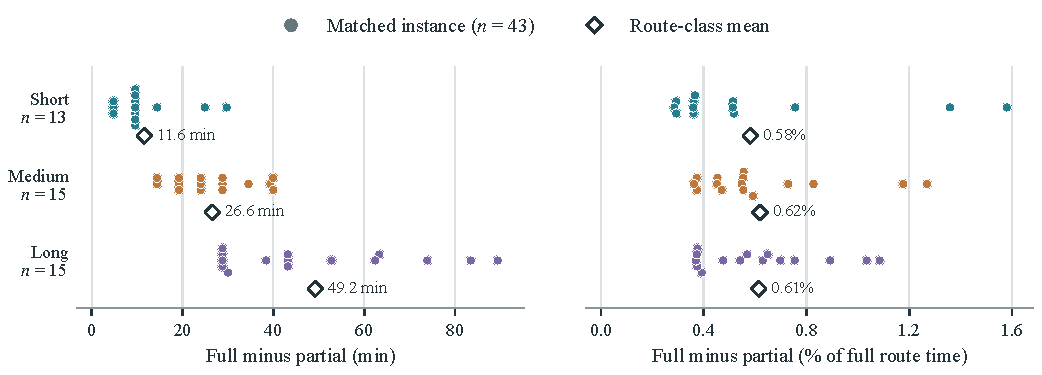
\includegraphics[width=\linewidth]{figures/paired_route_time.pdf}
    \caption{Base-case route duration under full charging minus route duration
    under partial charging, in minutes (left) and as a percentage of the
    full-charging duration (right). Dots represent individual matched
    instances and diamonds mark route-class means. Battery capacity is 750~kWh, charging
    power is 350~kW, station spacing is 60~km, and energy consumption is
    1.49~kWh/km. Station service per charging stop is 4.8~min under full
    charging and zero under partial charging.}
    \label{fig:paired_route_time}
\end{figure}

Figure~\ref{fig:charging_example} shows the battery profiles under both
charging policies and the breakdown of the route-time difference by
activity for \texttt{long\_cl3\_cu4\_Unbalanced}.

\begin{figure}[tbp]
    \centering
    \begin{subfigure}[b]{0.52\linewidth}
        \centering
        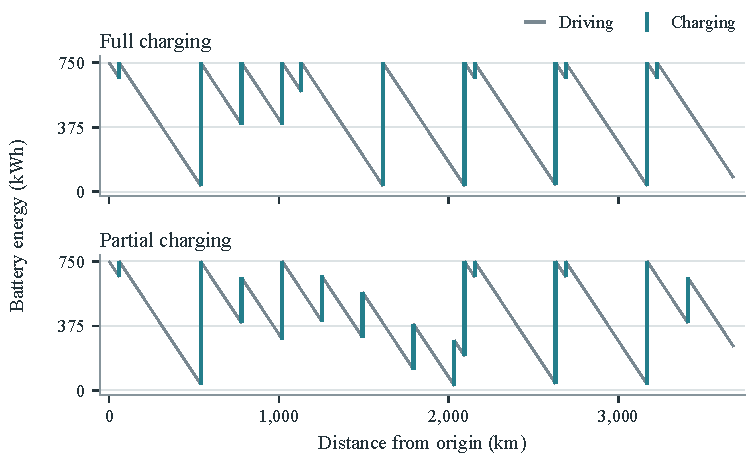
\includegraphics[width=\linewidth]{figures/battery_profiles.pdf}
        \caption{}\label{fig:battery_profiles}
    \end{subfigure}\hfill
    \begin{subfigure}[b]{0.46\linewidth}
        \centering
        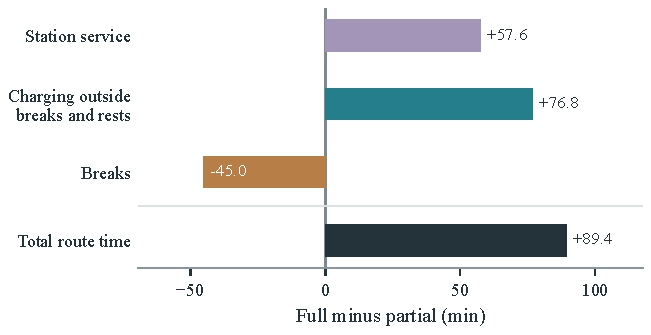
\includegraphics[width=\linewidth]{figures/time_breakdown.pdf}
        \caption{}\label{fig:time_breakdown}
    \end{subfigure}
    \caption{Full and partial charging on \texttt{long\_cl3\_cu4\_Unbalanced},
    the base-case instance with the largest recorded route-time difference
    (89.4~min). Panel~(a) shows battery energy along the route. Vertical
    segments show energy added at charging stops. Panel~(b) shows each
    activity's contribution to the difference in route time. Positive values
    indicate more time under full charging.}
    \label{fig:charging_example}
\end{figure}
